\documentclass{article}
\usepackage{amsmath}
\usepackage{amssymb}
\usepackage[a4paper, top=25mm, bottom=25mm, left=25mm, right=25mm]{geometry}
\usepackage{pgfplots}
\usepackage{polynom}
\usepackage{mathtools}
\pgfplotsset{compat=1.18}

\begin{document}
\pagestyle{empty}
\large

\begin{center}
2017-2018 Summer\\MAT123-07 Midterm\\(24/07/2018)
\end{center}

\noindent 1) Evaluate

\[\lim_{x\to3^+}(x-3)^{\ln(x-2)}\]

\hfill

\noindent 2) Find constants a and b such that $f(2) + 3 = f(0)$ and $f(x)$ is continuous at $x=1$ where $f(x)$ is defined by

\[
f(x) =
\begin{cases}
ax + b, & \text{if}\ x > 1 \\
3, & \text{if}\ x = 1 \\
x^2-4x+b+3, & \text{if}\ x < 1 \\
\end{cases}
\]

\noindent and $f(x)$ is continuous everywhere.

\hfill

\noindent 3) The top of a ladder leaning against a wall slides down the wall at the rate of 6 m/s. When the bottom of the ladder is 9 m from the wall, it is moved away from the wall at the rate of 5 m/s. How long is the ladder?

\hfill

\noindent 4) Sketch the graph of

\[f(x) = \frac{x^2+1}{x}\]

\hfill

\noindent 5) Evaluate the following integrals.

\hfill

\noindent (a) $\displaystyle \int\sqrt{4-\sqrt{x}}\, dx$

\hfill

\noindent (b) $\displaystyle \int(\ln x)^2\, dx$

\hfill

\noindent 6) Let us consider the area $A$ of the region bounded by the curve $x=y^2-6y$ and the straight line $x=-y$. Write an integral (but don't evaluate) corresponding to the area $A$

\hfill

\noindent (i) with respect to the $y$-axis and

\hfill

\noindent (ii) with respect to the $x$-axis.

\hfill

\newpage

\begin{center}
2017-2018 Summer Midterm (24/07/2018) Solutions\\
(Last update: 8/21/25 (21st of August) 3:07 PM)
\end{center}

\noindent 1) Let $L$ be the limit value. Then, take the logarithm of both sides.

\[L = \lim_{x\to3^+}(x-3)^{\ln(x-2)}\]

\[\ln(L) = \ln\left[\lim_{x\to3^+}(x-3)^{\ln(x-2)}\right]\]

\hfill

\noindent The function is continuous for $x > 3$. So, we can take the logarithm function inside the limit. Using the property of logarithms, we get:

\[\ln(L) = \lim_{x\to3^+}\ln\left[(x-3)^{\ln(x-2)}\right] = \lim_{x\to3^+}\left[\ln(x-2)\cdot \ln(x-3)\right]\]

\hfill

\noindent If we substitute $x=3$, we see that $\ln(1) = 0$. However, $\ln(x-3)$ becomes undefined (in other words, tends to negative infinity as $x\to3^+$). We can apply L'Hôpital's rule if we treat these two expressions as a single fraction. Rewrite the limit as follows:

\[\lim_{x\to3^+}\left[\ln(x-2) \cdot \ln(x-3)\right] =\lim_{x\to3^+}\left[\frac{\ln(x-2)}{\frac{1}{\ln(x-3)}}\right]  \]

\hfill

\noindent The limit is now in the form $\infty/\infty$. Apply the rule where indeterminate forms occur.

\begin{align*}
    \lim_{x\to3^+}\left[\frac{\ln(x-2)}{\frac{1}{\ln(x-3)}}\right] &\overset{\text{L'H.}}{=} \lim_{x\to3^+} \left[\frac{\frac{1}{x-2}}{-\frac{1}{\ln^2(x-3)}\cdot {\frac{1}{x-3}}}\right] = \lim_{x\to3^+} \left[-\frac{\ln^2(x-3)}{\frac{x-2}{x-3}}\right] \quad \left[\frac{\infty}{\infty}\right] \\\\
    &\overset{\text{L'H.}}{=} \lim_{x\to3^+}\left[-\frac{2\ln(x-3)\cdot\frac{1}{x-3}}{\frac{(x-3) -(x-2)}{(x-3)^2}}\right] = \lim_{x\to3^+} \left[\frac{2\ln(x-3)}{\frac{1}{x-3}}\right] \quad \left[\frac{\infty}{\infty}\right] \\\\
    &\overset{\text{L'H.}}{=} \lim_{x\to3^+} \left[\frac{\frac{2}{x-3}}{-\frac{1}{(x-3)^2}}\right] = \lim_{x\to3^+} \left[-\frac{2(x-3)}{1}\right]=\lim_{x\to3^+} (6-2x)\\\\&=0
\end{align*}

\hfill

\noindent Recall that we evaluated $\ln(L) = 0$, so $\boxed{L = 1}$.

\hfill

\noindent 2) We need to ensure continuity at $x=1$. The one-sided limits must be equal to the value of the function at that point. The function is a polynomial expression for $x<1$, and another polynomial expression for $x>1$. Both expressions are defined for $x=1$ (x=1 is actually in the domain with another condition), so we can just substitute $x=1$ in the limits.

\[\lim_{x\to1^+} (ax+b) = a+b = 3\]
\[\lim_{x\to1^-} (x^2-4x+b+3) = 1^2 -4 +b+3 =  3\]

\noindent $\boxed{b=3}$, so $a+3 = 3\rightarrow \boxed{a = 0}$.

\hfill

\noindent \textbf{Remark}: Condition $f(2) + 3 = f(0)$ is redundant because we already found the values of $a$ and $b$. It does not provide any further useful information, and it is unknown why it was included in the question.

\hfill

\noindent 3) Let $x = f(t), \,y = g(t)$ and $L$ be the length of the ladder. $f(t)$ and $g(t)$ represent the location of the bottom and top of the ladder, respectively. The length of the ladder remains constant as time goes on. We can write the following using the Pythagorean theorem. Apply the Chain Rule appropriately.

\[L = \sqrt{f^2(t) + g^2(t)}\]

\[\frac{dL}{dt} = \frac{d}{dt}\sqrt{f^2(t) + g^2(t)}\]

\[0 = \frac{1}{2\sqrt{f^2(t)+g^2(t)}} \cdot [2f(t)f'(t) + 2g(t)g'(t)]\]

\begin{equation}\therefore \, f(t)f'(t) = -g(t)g'(t)\end{equation}

\hfill

\noindent For $t=t_0$, given $g(t_0) = 9$ m, $f'(t_0) = -6$ m/s, $g'(t_0) = 5$ m/s. Find $f(t_0)$ using $(1)$.

\[f(t_0) = -\frac{g(t_0)g'(t_0)}{f'(t_0)} = -\frac{9\cdot (-5)}{6} = \frac{15}{2}\]

\noindent Now, we can find $L$.

\[L =\sqrt{f^2(t_0) + g^2(t_0)} = \sqrt{\left(\frac{15}{2}\right)^2 + 9^2} = \sqrt{\frac{549}{4}}\]

\hfill

\[\boxed{L=\frac{3\sqrt{61}}{2}}\]

\hfill

\noindent 4) First off, find the domain. The expression is undefined when the denominator is zero. Therefore, $x^2 \neq 0 \,\rightarrow\, x\neq0$. The only vertical asymptote occurs at $x = 0$.

\[\mathcal{D} = \mathbb{R} - \{0\} \]

\noindent Let us find the limit at infinity.

\[\lim_{x\to \infty} \frac{x^2+1}{x} \overset{\text{L'H.}}{=} \lim_{x\to \infty} \frac{2x}{1} = \infty\]

\noindent Similarly,

\[\lim_{x\to -\infty} \frac{x^2+ 1}{x} = -\infty\]

\hfill

\noindent There is no horizontal asymptote. However, there exists a slant asymptote. If we attempt to make a long division, the quotient will be $x$. So, the slant asymptote is $y=x$. Let us verify with the limit.

\[\lim_{x\to\infty} \left(\frac{x^2+1}{x} - x\right) = \lim_{x\to\infty} \frac{1}{x} = 0\]

\hfill

\noindent Take the first derivative by applying the quotient rule.

\[y' = \frac{2x\cdot x - (x^2+1)}{x^2}=\frac{x^2-1}{x^2}\]

\hfill

\noindent $y'$ is undefined for $x=0$, and $y'=0$ for $x=\pm1$. Since 0 is not in the domain, the \textit{only} critical points are $x=\pm 1$.

\hfill

\noindent Take the second derivative.

\[y'' = \frac{2x\cdot x^2 - (x^2-1)\cdot(2x)}{x^4}=\frac{1}{x^3}\]

\hfill

\noindent There is no inflection point because $\displaystyle \frac{1}{x^3} \neq 0, \, \forall x \in \mathbb{R}$.

\hfill

\noindent Consider some values of the function. Eventually, set up a table and see what the graph looks like in certain intervals.

\[f(-1) = \frac{(-1)^2 + 1}{-1} = -2,\quad f(1) = \frac{(1)^2 + 1}{1} = 2\]

\begin{center}
    \large
    \begin{tabular}{ |c| c c c c| } 
    \hline
        $x$ & $(-\infty, -1)$ & $(-1, 0)$ & $(0, 1)$ &  $(1, \infty)$ \\
        \hline
        $y$ & $(-\infty, -2)$ & $(-\infty, -2)$ & $(2, \infty)$ & $(2, \infty)$\\
        \hline
        $y'$ sign & + & - & - & + \\
        \hline
        $y''$ sign & - & - & + & + \\
        \hline
    \end{tabular}
\end{center}

\hfill

\begin{center}
\begin{tikzpicture}
  \begin{axis}[
    axis lines = center,
    xlabel = $x$, ylabel = $y$,
    domain=-5:5,
    samples=300,
    ymin=-5, ymax=5,
    xmin=-5, xmax=5,
    restrict y to domain=-6:6,
    enlargelimits=true,
    axis line style={->},
    ytick={-6,-4,-2,2,4,6},
    xtick={-6,-5,-4,-3,-2,-1, 1,2,3,4,5,6},
    scale=1.5,
    ]
    \addplot[blue, thick] {(x^2+1)/x};

    \draw[dashed, red] (axis cs:-5,-5) -- (axis cs:5,5);
    \draw[dashed, red] (axis cs:0.04,-6) -- (axis cs:0.04,6);
    \draw[dashed, black] (axis cs:0,2) -- (axis cs:1,2);
    \draw[dashed, black] (axis cs: 0,-2) -- (axis cs:-1,-2);
    \draw[dashed, black] (axis cs:1,0) -- (axis cs:1,2);
    \draw[dashed, black] (axis cs: -1,0) -- (axis cs:-1,-2);

  \end{axis}
\end{tikzpicture}
\end{center}

\newpage

\noindent 5)

\hfill

\noindent (a) Let $u=\sqrt{4-\sqrt x}$.

\[u^2=4-\sqrt x\implies 4-u^2=\sqrt x\implies\left(4-u^2\right)^2=x\implies2\left(4-u^2\right)\cdot(-2u)\,du=dx\]

\begin{align*}\int\sqrt{4-\sqrt{x}}\,dx&=\int u\cdot(8-2u^2)\cdot(-2u)\,du=\int\left(4u^4-16u^2\right)\,du=\frac{4u^5}5-\frac{16u^3}3+c\\\\&=\boxed{\frac{4\left(\sqrt{4-\sqrt x}\right)^5}5-\frac{16\left(\sqrt{4-\sqrt x}\right)^3}3+c,\quad c\in\mathbb{R}}\end{align*}

\hfill

\noindent (b) Apply integration by parts.

\[\left.\begin{array}{c}
u=(\ln x)^2\implies du=2\ln x\cdot\dfrac1x\,dx\\
dv=dx\implies v=x
\end{array}\right\}\rightarrow \int u\,dv=uv-\int v\,du\]

\[\int(\ln x)^2\,dx=x(\ln x)^2-\int2\ln x\,dx\]

\hfill

\noindent Apply integration by parts once again.

\[\left.\begin{array}{c}
u=\ln x\implies du=\dfrac1x\,dx\\
dv=dx\implies v=x
\end{array}\right\}\rightarrow \int u\,dv=uv-\int v\,du\]

\[\int(\ln x)^2\,dx=x(\ln x)^2-\int2\ln x\,dx\]

\[x(\ln x)^2-\int2\ln x\,dx=x(\ln x)^2-2\left[x\ln x-\int dx\right]=\boxed{x(\ln x)^2-2x\ln x+2x+c,\: c\in\mathbb{R}}\]

\hfill

\noindent 6)

\begin{center}
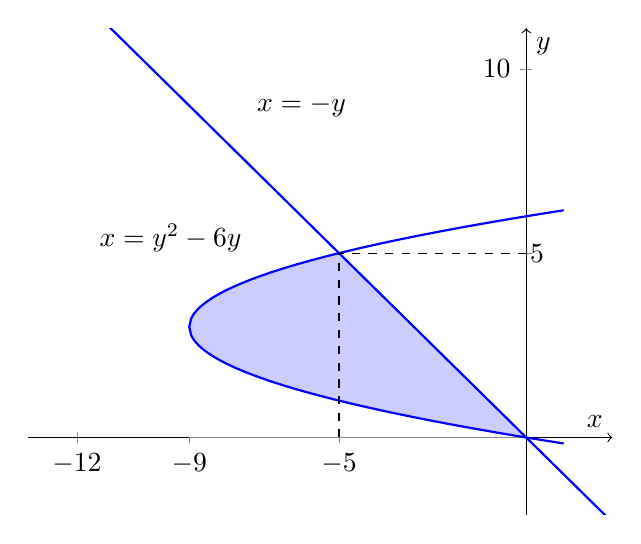
\begin{tikzpicture}
  \begin{axis}[
  width=9cm,
    yticklabel pos=right,
    axis lines = center,
    xlabel = $x$, ylabel = $y$,
    domain=-12:4,
    samples=300,
    ymin=-1, ymax=10,
    xmin=-12, xmax=1,
    enlargelimits=true,
    axis line style={->},
    ytick={10},
    xtick={-12, -9, -5},
    extra y ticks={5},
    extra y tick labels={5},
    extra y tick style={
        yticklabel pos=right,
        ticklabel style={anchor=west},
    },
    ]
    \addplot [
      domain=-9:-5,
      samples=200,
      fill=blue!20,
      draw=none,
    ]
    {sqrt(x+9)+3} \closedcycle;
    
    \addplot [
      domain=-5:0,
      samples=200,
      fill=blue!20,
      draw=none,
    ]
    {-x} \closedcycle;

    \addplot [
      domain=-9:0,
      samples=200,
      fill=white,
      draw=none,
    ]
    {-sqrt(x+9)+3} \closedcycle;
    
    \addplot[blue, thick, domain=-9:1, samples=200] {sqrt(x+9) + 3};
    \addplot[blue, thick, domain=-9:1, samples=200] {-sqrt(x+9) + 3};
    \addplot[blue, thick] {-x};

    \node at (axis cs:-6,9) {$x=-y$};
    \node at (axis cs:-9.5,5.4) {$x=y^2-6y$};

    \draw[dashed, black] (axis cs:-5,0) -- (axis cs:-5,5);
    \draw[dashed, black] (axis cs:0,5) -- (axis cs:-5,5);
  \end{axis}
\end{tikzpicture}\hspace{0.5cm}
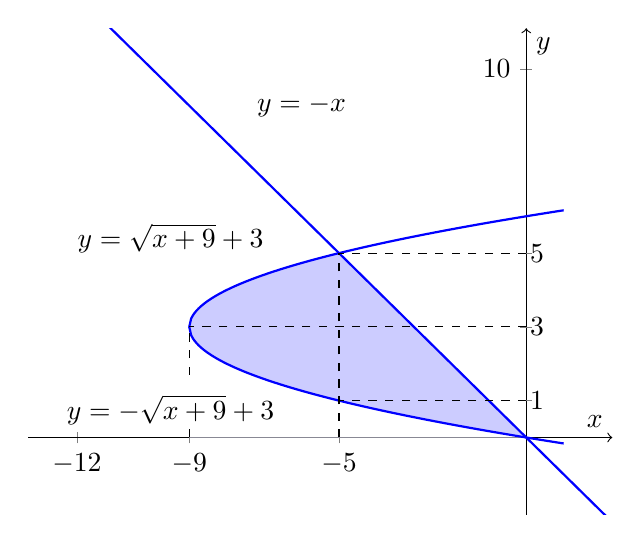
\begin{tikzpicture}
  \begin{axis}[
    width = 9cm,
    yticklabel pos=right,
    axis lines = center,
    xlabel = $x$, ylabel = $y$,
    domain=-12:4,
    samples=300,
    ymin=-1, ymax=10,
    xmin=-12, xmax=1,
    enlargelimits=true,
    axis line style={->},
    ytick={10},
    xtick={-12, -9, -5},
    extra y ticks={5,3,1},
    extra y tick labels={5,3,1},
    extra y tick style={
        yticklabel pos=right,
        ticklabel style={anchor=west},
    },
    ]
    \addplot [
      domain=-9:-5,
      samples=200,
      fill=blue!20,
      draw=none,
    ]
    {sqrt(x+9)+3} \closedcycle;
    
    \addplot [
      domain=-5:0,
      samples=200,
      fill=blue!20,
      draw=none,
    ]
    {-x} \closedcycle;

    \addplot [
      domain=-9:0,
      samples=200,
      fill=white,
      draw=none,
    ]
    {-sqrt(x+9)+3} \closedcycle;
    
    \addplot[blue, thick, domain=-9:1, samples=200] {sqrt(x+9) + 3};
    \addplot[blue, thick, domain=-9:1, samples=200] {-sqrt(x+9) + 3};
    \addplot[blue, thick] {-x};

    \node at (axis cs:-6,9) {$y=-x$};
    \node at (axis cs:-9.5,5.4) {$y=\sqrt{x+9} + 3$};
    \node at (axis cs:-9.5,0.75) {$y=-\sqrt{x+9} + 3$};

    \draw[dashed, black] (axis cs:-5,0) -- (axis cs:-5,5);
    \draw[dashed, black] (axis cs:0,3) -- (axis cs:-9,3);
    \draw[dashed, black] (axis cs:0,1) -- (axis cs:-5,1);
    \draw[dashed, black] (axis cs:0,5) -- (axis cs:-5,5);
    \draw[dashed, black] (axis cs:-9,0) -- (axis cs:-9,0.3);
    \draw[dashed, black] (axis cs:-9,1.7) -- (axis cs:-9,3);

  \end{axis}
\end{tikzpicture}
\end{center}

\hfill

\noindent (i) We'll take the integral along the $y$-axis. The lower and upper limits of the integral are 0 and 5, respectively.

\[A = \int_0^5[(-y)-(y^2-6y)]\,dy = \int_0^5(-y^2+5y)\,dy\]

\hfill

\noindent (ii) We have two different regions. $y=-x$ and $y=\sqrt{x-9}+3$ intersect at the point $(-5, 5)$. Therefore, we will write two separate integrals.

\begin{align*}
A&=\int_{-9}^{-5}\left[\left(\sqrt{x+9}+3\right) -\left(-\sqrt{x+9}+3\right)\right]\,dx + \int_{-5}^{0}\left[(-x) - \left(-\sqrt{x+9}+3\right)\right]\,dx\\\\
&=\int_{-9}^{-5}2\left(\sqrt{x+9}\right)\,dx + \int_{-5}^{0}\left(-x + \sqrt{x+9}-3\right)\,dx
\end{align*}

\end{document}